\section{Implementation} \label{sec:impl}
In this section, we present the implementation details of the \module and the \cache based on Linux (the guest kernel) and Xen (the hypervisor).

\subsection{\name Module}
\begin{figure}[ht]
\centering
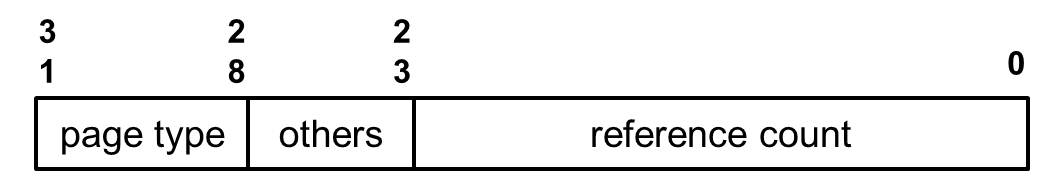
\includegraphics[width=0.45\textwidth]{image/implementation/field-of-page-type-info.jpg} \\
\caption{The layout of the original data structure for page type.}
\label{fig:field-of-page-type-info}
\end{figure}
The first main task of the \module is to extend the existing data structures to support semi-writable page table.
As illustrated in Figure~\ref{fig:field-of-page-type-info}, the data structure for labelling page types is 32bits, i.e., bits 28 - 31 are allocated for page type, bits 23 - 27 is for others (e.g., bit 26 indicate if this page has been validated), and bits (0 - 22) is for reference count.
The existing page types have occupied all page type bits, and there is no extra bit for semi-writable page.
Facing this problem, we do not choose to introducing new data structures, as it would increase the management complexity and result in many modifications of all related management functions.
Instead, we choose to borrowing a bit from \emph{reference count}.
In particular, the \emph{reference count} field has 23 bits, presenting how many references on a page. 
In fact, the system usually does not build so many references on one page. Thus, we borrow the highest bit (bit 22) as the semi-page table bit (as illustrated in Figure~\ref{fig:field-of-semi-type}).
As a consequence, it still supports more than 4 million reference counts, enough for almost all cases. 
Actually, the hypervisor is functioning well in our experiments.

The \module also needs to patch the page type checking functions, e.g., \_\_get\_page\_type, to adjust the checking logic. 
The added checking logic is straightforward, such that we only add 166 SloC to achieve the whole patch.
In addition, some validation steps (e.g., DMA validations) necessary before could be skipped when the semi-writable page is involved in the page type update, simplifying the whole validation logic in a certain level. 

\begin{figure}[ht]
\centering
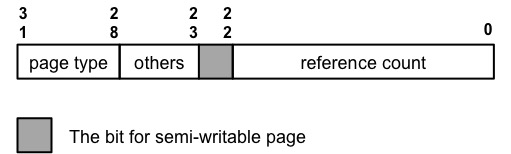
\includegraphics[width=0.45\textwidth]{image/implementation/field-of-semi-type.jpg} \\
\caption{The semi-writable page type support.}
\label{fig:field-of-semi-type}
\end{figure}

\subsection{\name Cache}
%data structures
There are three levels of the guest page table, and the \cache maintains a single-linked list for each of them.
Each node of the list has a pointer pointing to the next node and a page ID that is the base address of a cached page.
Note that this address should be a physical address, rather than a virtual address, because physical address is unique in the whole system but its virtual addresses could have many.
Thus, using virtual address would lead to the confusion of the page type tracing and the semi-writable page management.
As the page table allocations and deallocations could happen at any time on any core, each list has its own lock and supports concurrent updates.

%interfaces
The \cache has two interfaces for the runtime page table allocations and deallocations.
The \emph{pop} interface is for the page table allocations.
When this interface is invoked, the \cache will fetch the top node of the corresponding list, extract the base address of the cache page, and then returns it to the caller.
Correspondingly, the \emph{push} interface is serving for the page table deallocations.
In the push interface, the \cache saves the base address of the deallocated page into a node, and inserts it on the top of the list.
Obviously, the pop and push interfaces are extremely fast as they could response to the allocation and deallocation requests in a constant time.

%provide interfaces for end user
The \cache also add several files in \emph{sysfs} that is a virtual file system provided by the Linux kernel. 
By using the virtual files, the end user could send command to the \cache, as well as query and configure the internal status.
In the current implementation, we only support one command, which is able to activate and deactivate the cache service in an on-demand way.
In addition, the end user could use the new interface to query the number of the cached pages, and dynamically shrink the cache size. 
For instance, the end user could explicitly ask the \cache to release all the cached pages by setting the number of the cached pages to be zero.

% handle cache shrinking and page type update
The \cache mediates all page type updates related to the semi-writable pages. 
For each page type update, the \cache would issue the hypercall exported by the \module to explicitly inform the hypervisor to perform security validations.
In certain cases, such as shrinking the cached semi-writable pages to writable pages, the \cache could submit a batch of requests through the hypercall.
In such cases, the hypervisor would update the I/O page tables as well as flush IOTLBs in one time, saving time for the cache shrinking.








